\documentclass[12pt,%
addpoints,%
%answers%
]{exam}

\usepackage[french]{babel}
\usepackage[utf8]{inputenc}
\usepackage{graphicx}
\usepackage{subcaption}
\usepackage{dejavu}
\renewcommand*\familydefault{\sfdefault} %% Only if the base font of the document is to be sans serif
\usepackage[T1]{fontenc}

\usepackage{geometry}
\geometry{a4paper,headheight=16pt,tmargin=25mm,
          bmargin=25mm,lmargin=20mm,rmargin=20mm}

\usepackage{lastpage}
\usepackage{hyperref}
\usepackage{array}
\usepackage{minted}
\usepackage{tcolorbox}
\usepackage{xcolor}

\footer{ENSEA}{Page~\thepage/\pageref{LastPage}}{TP Linux Embarqué}

\newcommand{\new}[1]{\textcolor{red}{\textbf{#1}}}

\title{TP Systèmes à microprocesseurs}
\date{}

\begin{document}
 \begin{center}
	 {\LARGE\bfseries\sffamily TP Systèmes à microcontrôleurs}
	 \vspace{1em}
  \par\bigskip
\end{center}

L'objectif de ce TP en 4 séances est de concevoir, assembler et tester une carte électronique contenant un microcontrôleur STM32.
Le TP a été conçu avec la version 6.0.9 de KiCAD, mais devrait être réalisable avec d'autres versions.\\

Cette carte sera constituée des composants suivants :
\begin{itemize}
	\item Microcontrôleur STM32L021K4T6, 
	\item DAC MCP4801-E/SN,
	\item Régulateur linéaire BU33SD5WG-TR,
	\item 2 LED au format 0603,
	\item Connecteur de programmation FTSH-107-01-F-DV,
	\item Plusieurs composants passifs (résistances, condensateurs...) en 0603.\\
\end{itemize}

La carte est donc munie d'un ADC (intégré au MCU) et d'un DAC (composant externe sur la carte).
Pour démontrer le bon fonctionnement de la carte, vous programmerez un filtre numérique simple.

L'ordre des séances est le suivant:
\begin{enumerate}
	\item Schéma, association empreintes
	\item Routage du circuit
	\item Soudure, test...
	\item Écriture du firmware
\end{enumerate}

\setcounter{section}{-1}
\section{Utilisation de \texttt{git}}
Les outils de gestion de version permettent de travailler facilement à plusieurs sur du code, ou autre.
L'outil \texttt{git} est probablement le plus courant. C'est celui que nous allons utiliser.

Sous Linux, l'outil s'utilise simplement en ligne de commande. Sous Windows, il existe des outils. Je suis un Linuxien, débrouillez-vous.

\texttt{Git} est un outil puissant, complet et complexe, mais nous n'aurons besoin de connaître que 5 commandes :
\begin{itemize}
	\item \mintinline{bash}{git clone} : Cloner un projet, c'est la première étape pour récupérer son projet, ou n'importe quel projet publique.
	\item \mintinline{bash}{git pull} : Récupérer les dernières modifications
	\item \mintinline{bash}{git add <fichier>} : Enregistrer des fichiers auprès de git
	\item \mintinline{bash}{git commit -m "Message"} : Réaliser un commit, c'est à dire enregistrer les modifications locales. 
		On peut l'utiliser comme un verbe. Ex: "\emph{Oups, j'ai oublié de commiter mon code}".
	\item \mintinline{bash}{git push} : Pousser du code sur le serveur. Le commit se faisant localement, cette commande permet de pousser le commit sur le serveur.
\end{itemize}


\begin{tcolorbox}
	Je vous recommande \textbf{fortement} d'utiliser cet outil pour tout vos TP, que ce soit pour le code ou pour les compte-rendu.
\end{tcolorbox}

\begin{questions}
	\question Si ce n'est pas déjà fait, créez un compte (par étudiant) sur le site suivant :
\url{https://github.com/}
	\question Créez un nouveau \emph{repository}. Laissez-le en public. Vous pouvez ajouter une description et un fichier \texttt{README}.
	\question Récupérez l'adresse du projet. Cliquez sur \texttt{Code}, choisissez \texttt{SSH}, puis copiez l'adresse.
	\begin{center}
		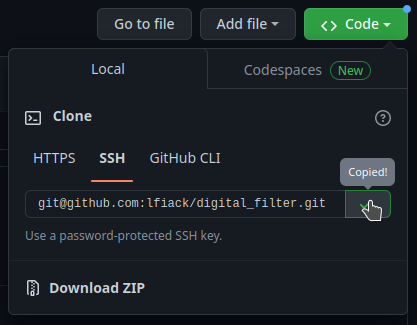
\includegraphics[width=.5\linewidth]{figures/git1.png}
	\end{center}
	\question Clonez le projet. Dans un terminal, tapez la commande suivante : \\
		\mintinline{bash}{git clone <adresse_du_depot>}.
	\question Modifiez le fichier \texttt{README}.
	\question Réalisez votre premier commit. Tapez les deux commandes suivantes : \\
	\mintinline{bash}{git add .}\\
	\mintinline{bash}{git commit -m "First!"}
	\question Poussez les modifications sur le \texttt{repository} distant : \\
	\mintinline{bash}{git push}
	\question Vérifiez que les modifications ont bien été prises en compte sur \url{https://github.com/}
\end{questions}

\begin{tcolorbox}
	Quelques bonnes pratiques :
	\begin{itemize}
		\item Faire un \mintinline{bash}{git pull} au début de chaque session de travail (on sait jamais, peut-être que mon binôme a travaillé?)
		\item Commiter régulièrement :
			\begin{itemize}
				\item Dès que quelque chose fonctionne
				\item À la fin de la session de travail
				\item Éviter de commiter du code qui plante (à l'école, ça peut entrer en contradiction avec le point précédent...)
				\item Mettez un message utile!
			\end{itemize}
		\item Utiliser le fichier README comme document de travail.
	\end{itemize}
\end{tcolorbox}

\section{Saisie du schéma}
\subsection{Création de la structure du projet}
Le projet contiendra du hardware et du software. Il est impératif de bien structurer le dossier de travail.
%% Git?
\begin{questions}
	\question Dans le dossier \texttt{git}, créez un dossier \texttt{hardware}, un dossier \texttt{firmware} et un dossier \texttt{datasheets}.
	\question Téléchargez les \emph{datasheets} de tous les composants, et copiez les dans le dossier \texttt{datasheets}. 
		Attention, la documentation du STM32 est en plusieurs parties.
		Téléchargez également la \emph{datasheet} de la sonde de programmation STLINK-V3MINI. Pensez à commiter.
	\question Lancez STM32CubeMX. C'est un outil pratique lors de la conception d'une carte, notamment pour gérer le \emph{pinout}.
	\question Créez un projet pour le \texttt{STM32L021K4}. 
	\question Dans \texttt{SYS}, activez \texttt{Debug Serial Wire}.
	\question Activez l'\texttt{USART2} en mode \texttt{Asynchrone}. Gardez les paramètres par défaut, et notez le \texttt{baud rate}.
	\question Dans l'onglet \texttt{Clock Configuration}, configurez l'horloge système à sa valeur maximale.
	\question Dans \texttt{Project Manager > Code Generator}, cochez \texttt{Generate peripheral initialization as a pair of '.c/.h' files per peripheral}
	\question Sauvegardez dans le dossier \texttt{firmware}. L'initialisation n'est pas terminée, vous y reviendrez en temps voulu.
	\question Pensez à commiter.
\end{questions}

\subsection{Le microcontrôleur sous KiCAD}
\begin{questions}
	\question Lancez KiCAD. Créez un projet dans le dossier \texttt{hardware}.
	\question Cliquez sur \texttt{Place > Add symbol} (Vous pouvez commencer à apprendre les raccourcis.)
	\question Chechez et placez le composant STM32L021K4Tx.
	\question Cliquez sur \texttt{Place > Add Power} (Aussi présent dans le menu à droite.)
	\question Placer GND proche des \emph{pins VSS} du STM32, et câblez-les comme dans la capture ci-dessous.\\
	\begin{center}
	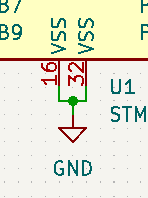
\includegraphics[width=.2\linewidth]{figures/kicad03.png} 
	\end{center}
	\question Ajouter deux autres symboles +3.3V et +3.3VA selon la capture ci-dessous.\\
	\begin{center}
    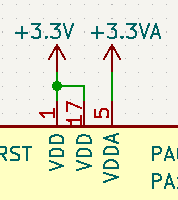
\includegraphics[width=.2\linewidth]{figures/kicad04.png}
    \end{center}
	\question Cliquez sur \texttt{Place > Add Label}
		Placez le label sur l'entrée NRST et nommez le NRST.

	\begin{center}
		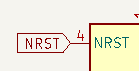
\includegraphics[width=.2\linewidth]{figures/kicad06.png}
	\end{center}

		Il sera plus tard relié au port de programmation.
		Deux signaux connectés à un même label sont reliés électriquement. Ça permet de simplifier la lecture du schéma.

	\question Ajoutez les labels correspondant aux signaux définis dans STM32CubeMX (USART2\_RX, USART2\_TX, SWDIO, SWDCLK). \\

		D'ailleurs, c'est peut-être le bon moment de finaliser le \emph{pinout}
	\question Activez l'entrée IN1 de l'ADC. Ce sera l'entrée analogique pour le filtre.
	\question Dans TIM2, mettez \emph{Clock Source} à \emph{Internal Clock} et \emph{Channel 1} à \emph{PWM Generation CH1}. 
		On s'en servira pour faire varier la luminosité de la LED.
	\question Enfin, configurez les signaux nécessaires pour l'utilisation du DAC.
		Le résultat final pourrait ressembler à ça:

	\begin{center}
        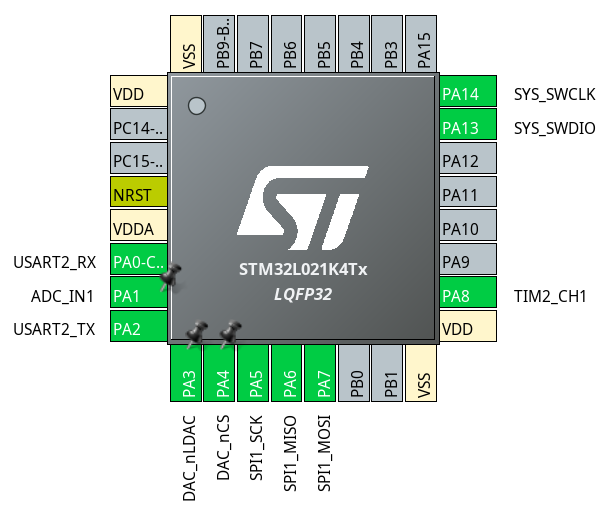
\includegraphics[width=.5\linewidth]{figures/cube01.png}
    \end{center}

		Sauvegardez.

\newpage

	\question Il est temps d'ajouter le reste des composants. Ajoutez les composants suivants:
	\begin{itemize}
		\item 6x C\_Small
		\item 1x L\_Small
		\item 2x R\_Small
		\item 1x LED\_Small\\
	\end{itemize}

		Le schéma correspondant à la partie microprocesseur pourrait ressembler à ça:

    \begin{center}
        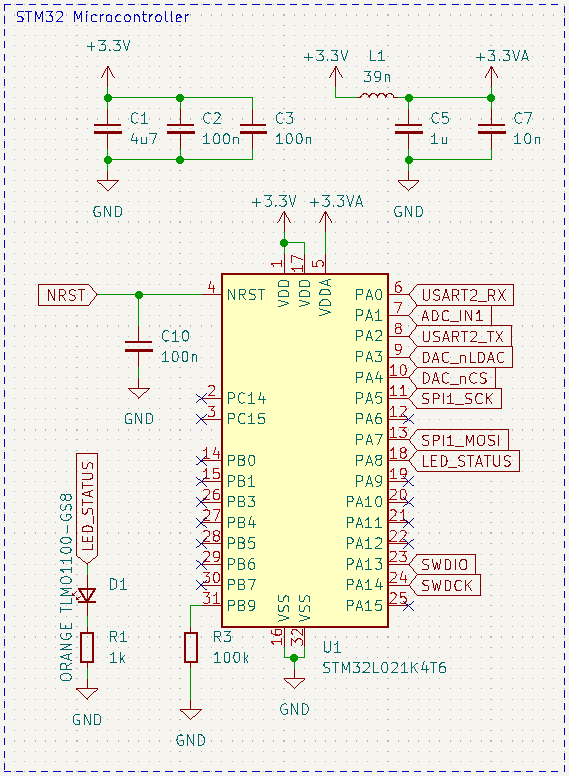
\includegraphics[scale=0.5]{figures/kicad07.png}
    \end{center}

		Notez qu'il n'est pas nécessaire d'annoter les composants à ce stade. Ce sera fait automatiquement plus tard.
		Les composants peuvent donc être nommés C?, L?, U?...

		Par contre, il est important de bien noter les valeurs des composants (4u7, 39n, 1k...)
	\question Pourquoi PB9 est relié à la masse? (Répondez à cette question, et aux suivantes, dans le README du repo git.)
	\question Quel est le rôle de L1, C5 et C7?
\end{questions}

\newpage

\subsection{Le reste du schéma}
Pour générer la tension de 3.3V à partir du 5V, nous utiliserons le régulateur linéaire LDO \texttt{BU33SD5WG-TR}.
Il n'est pas présent dans la librairie de KiCAD. 
Pour éviter d'avoir à dessiner un nouveau symbole, nous pouvons simplement utiliser un autre composant qui dispose du même boitier, comme le \texttt{MCP1802x-xx02xOT}.

\begin{questions}
	\question Ajouter le composant \texttt{MCP1802x-xx02xOT} et renommez-le en \texttt{BU33SD5WG-TR}
	\question Câblez le régulateur de tension en vous basant sur la figure suivante:
	\begin{center}
        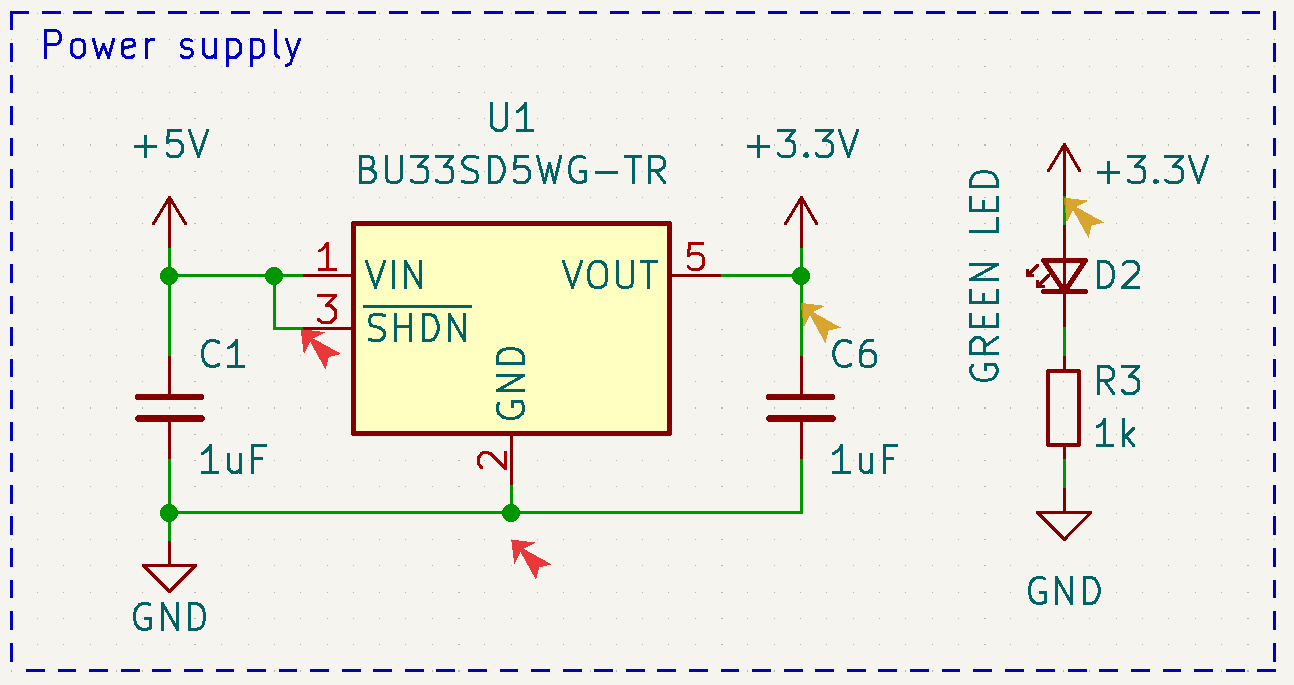
\includegraphics[scale=0.3]{figures/kicad08.png}
    \end{center}
	\question Quelle page de la \emph{datasheet} indique les valeurs des condensateurs?

	\question Tracez le schéma du DAC en vous inspirant de la figure suivante:
	\begin{center}
        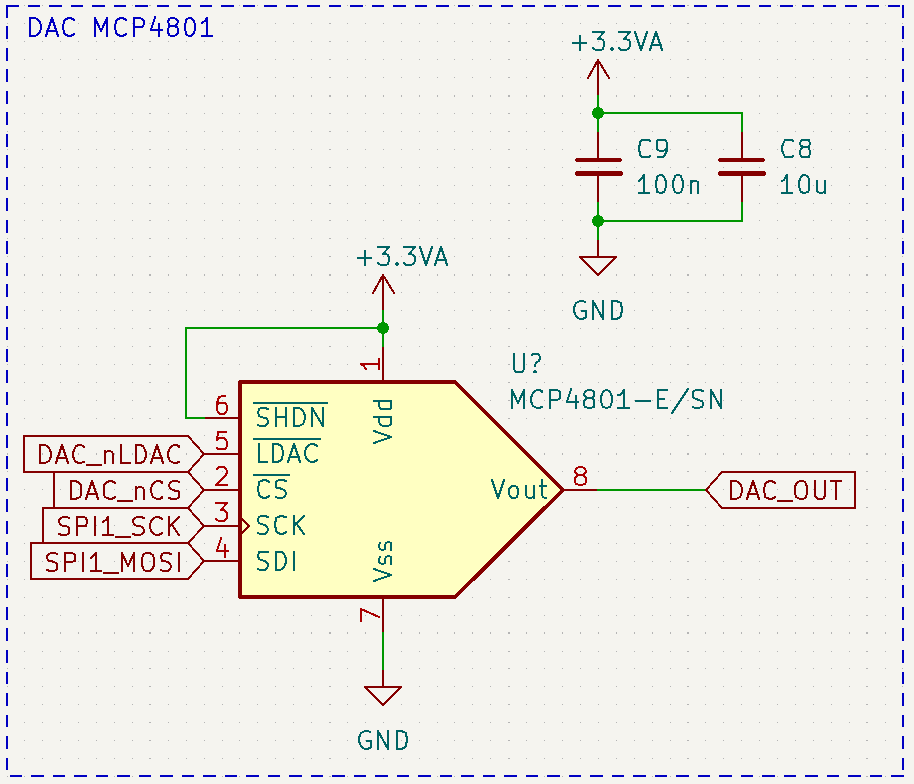
\includegraphics[scale=0.4]{figures/kicad09.png}
    \end{center}
	\question Quelle page de la \emph{datasheet} nous indique les valeurs de condensateurs?
	\question Quel est le rôle de la broche $\overline{\textrm{CS}}$?
	\question Quel est le rôle de la broche $\overline{\textrm{LDAC}}$?
	\question Pourquoi le signal $\textrm{MISO}$ n'est pas utilisé?

	\newpage
	\question Câblez les connecteurs comme dans la figure suivante:
	\begin{center}
        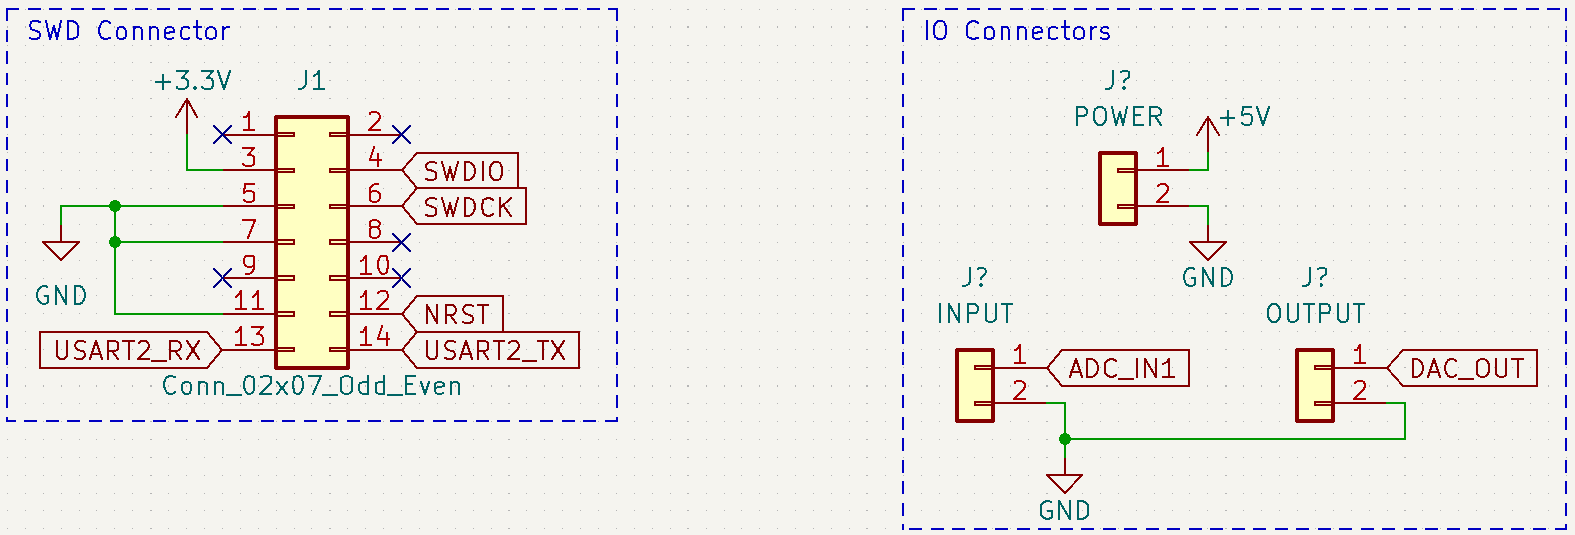
\includegraphics[scale=0.4]{figures/kicad10.png}
    \end{center}
	\question Où trouve-t-on les indications du pinout du connecteur SWD?

	\question Numérotez les composants en cliquant sur \texttt{Tools > Annotate Schematic...}

	\question Vérifiez les ERC (Electrical Rule Check) en cliquant sur \texttt{Inspect > Electrical Rules Checker}.
		
		Les erreurs suivantes peuvent être ignorées. S'il y en a plus, c'est qu'il y a peut-être des erreurs dans le schéma, corrigez les.
	\begin{center}
        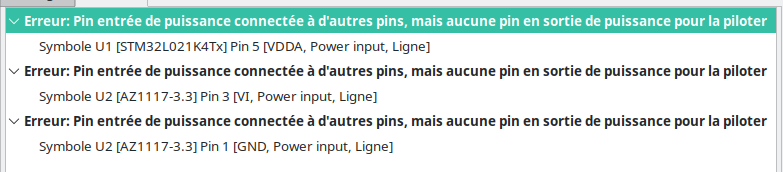
\includegraphics[width=\linewidth]{figures/kicad13.png}
    \end{center}
\end{questions}

\newpage
\subsection{Affectation des empreintes}
Vous avez fini le tracé du schéma. Il faut maintenant, pour chaque composant, associer un empreinte. 
\begin{questions}
	\question Cliquez sur \texttt{Tools > Assign Footprints...}
	\question Faire les associations selon la figure suivante. 
	Attention, en fonction du placement des composants dans le schéma, les composants n'ont peut-être pas les mêmes noms.
	\begin{center}
        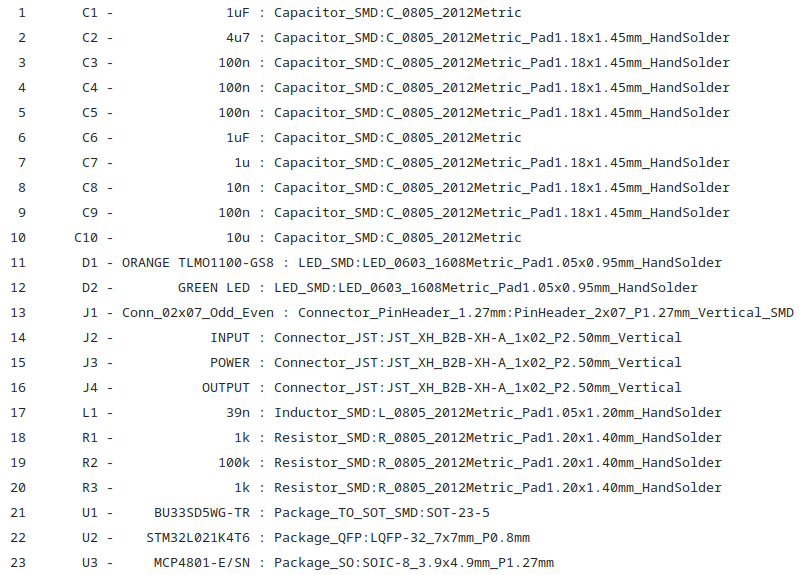
\includegraphics[width=\linewidth]{figures/kicad15.png}
    \end{center}

	Pour trouver plus facilement les empreintes, il peut être utile de bien configurer les filtres 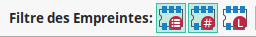
\includegraphics[height=2em]{figures/kicad16.png}

	\question Que signifie 0805? 0603? 1206?

	\question Que signifie LQFP? SOT-223? SOIC? Ne vous contentez pas de donner le sigle, j'attends une petite description (vous pouvez copier-coller depuis wikipedia, mais lisez avant quand même))
\end{questions}

\vspace{3em}

Félicitations! Vous avez tracé le schéma complet de votre circuit et avez associé une empreinte à chaque symbole dans le schéma.
Dans l'étape suivante, ces informations seront importées dans le logiciel de routage.

Faites vérifier le schéma à l'enseignant avant de passer à la suite.

\newpage

\section{Routage du circuit}
\subsection{Placement des composants}
\begin{questions}
	\question Ouvrez l'\emph{Éditeur de PCB}.
	\question Cliquez sur \texttt{Tools > Update PCB from Schematic...}

	Les composants sont mis en vrac, les connexions à router sont représentées par des traits fins.
	Cet ensemble de traits est appelé \emph{chevelu} (ou \emph{ratsnest} en Anglais).

	\begin{center}
        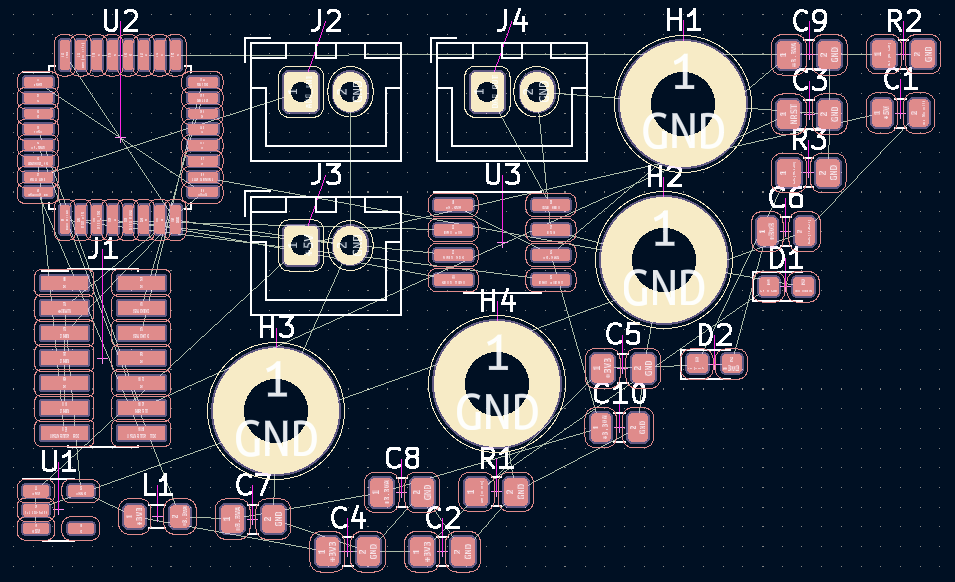
\includegraphics[width=.8\linewidth]{figures/kicad18.png}
    \end{center}

	Dans la figure ci-dessus, il y a 4 grandes pastilles que vous n'avez pas chez vous. 
	Elles serviront de trous de fixation. Il y a plusieurs méthodes pour les ajouter.
	Vous allez les rajouter dans le schéma.

	\question Dans l'\emph{Éditeur de Schématique}, ajouter les composants suivants:

	\begin{center}
        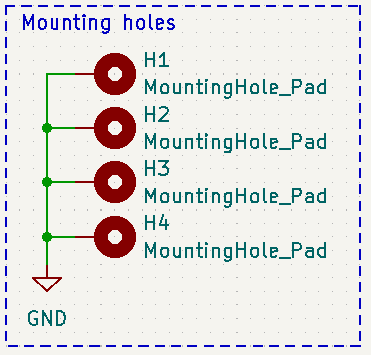
\includegraphics[scale=0.5]{figures/kicad19.png}
    \end{center}

	\question N'oubliez pas de faire le lien avec les empreintes :

	\begin{center}
        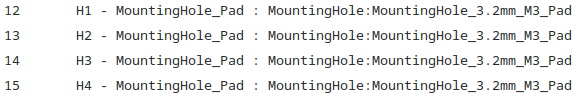
\includegraphics[width=.8\linewidth]{figures/kicad20.png}
    \end{center}

	\question Réglez la grille à 1mm.

	\question Commencez par placer les trous de fixation à 50mm de distance sur l'axe X et à 40mm de distance sur l'axe Y.

	\question Tracez les contours du circuit. Cliquez sur \texttt{Edge.Cuts} dans le panneau de droite. 
		Utilisez les lignes droites et les arcs de cercle pour obtenir quelque chose comme dans la figure suivante :

	\begin{center}
        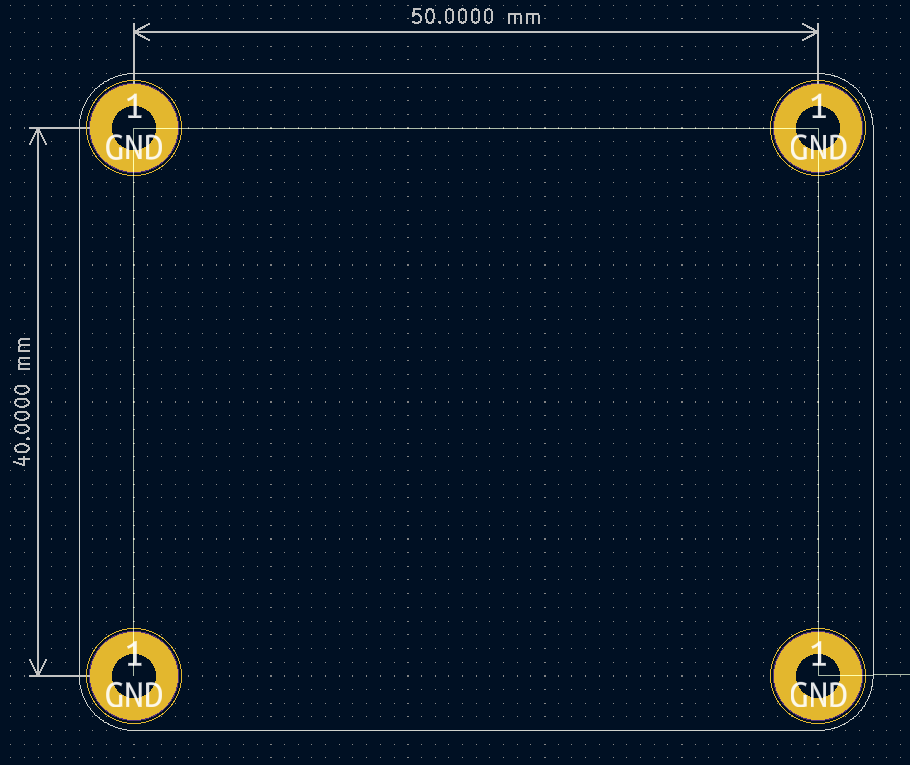
\includegraphics[width=.7\linewidth]{figures/kicad21.png}
    \end{center}

	\question Placez ensuite le connecteur d'alimentation au milieu en haut du circuit, à 4mm du bord.
	Placez le connecteur pour l'entrée analogique à gauche et le connecteur pour la sortie à droite.
	Voir la figure suivante :
	\begin{center}
        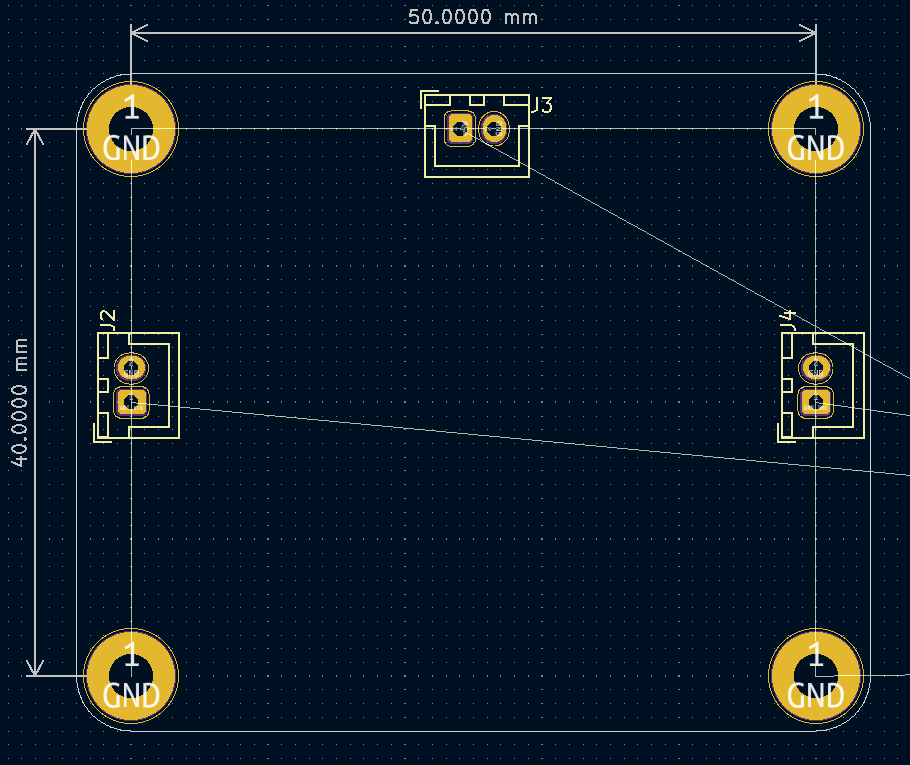
\includegraphics[width=.7\linewidth]{figures/kicad22.png}
    \end{center}

	\question Cliquez sur \emph{Placer > Origine des Coord de Perçage/Placement}. Positionnez l'origine sur l'un des trous de fixation.
	Cette étape est nécessaire pour la fabrication.

	\question Pour améliorer la lisibilité, vous pouvez masquer les couches \texttt{F.Fab} et \texttt{B.Fab} 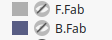
\includegraphics[height=2em]{figures/kicad23.png}

	\question Placez les composants. Pour faciliter le routage, il y a quelques règles à respecter.
	\begin{itemize}
		\item Placer le composant le plus complexe (le STM32) au centre.
		\item Placer les condensateurs de découplage proche des broches d'alimentation à découpler.
		\item Avoir le schéma ouvert dans une autre fenêtre, sur un autre écran de préférence.
		\item Essayer de réduire au maximum les croisements dans le chevelu.
		\item Prendre son temps. Ne pas hésiter à retourner à cette étape si le routage est compliqué.
	\end{itemize}

	Une fois les composants placés, faites vérifier par l'enseignant avant de passer à la suite.
\end{questions}

\subsection{Routage}
Avant de commencer à router, il faut configurer les règles de routage pour s'assurer que le circuit soit fabricable.
\begin{questions}
	\question Cliquez sur \texttt{File > Board Setup...}
	\question Dans \emph{Design Rules > Constraints}, configurez selon la figure suivante:
	\begin{center}
        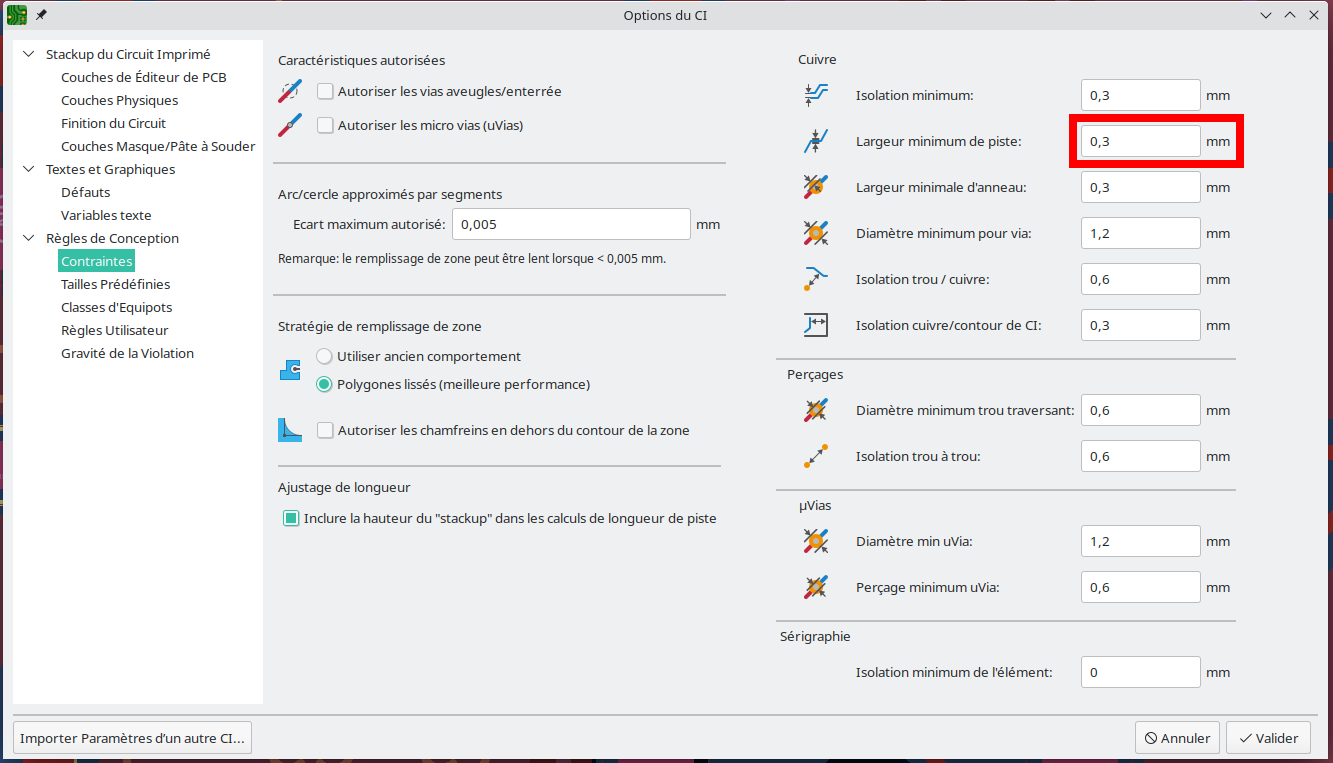
\includegraphics[width=\linewidth]{figures/kicad25.png}
    \end{center}

	\newpage

	\question Dans \emph{Design Rules > Pre-defined Sizes}, configurez selon la figure suivante:
	\begin{center}
        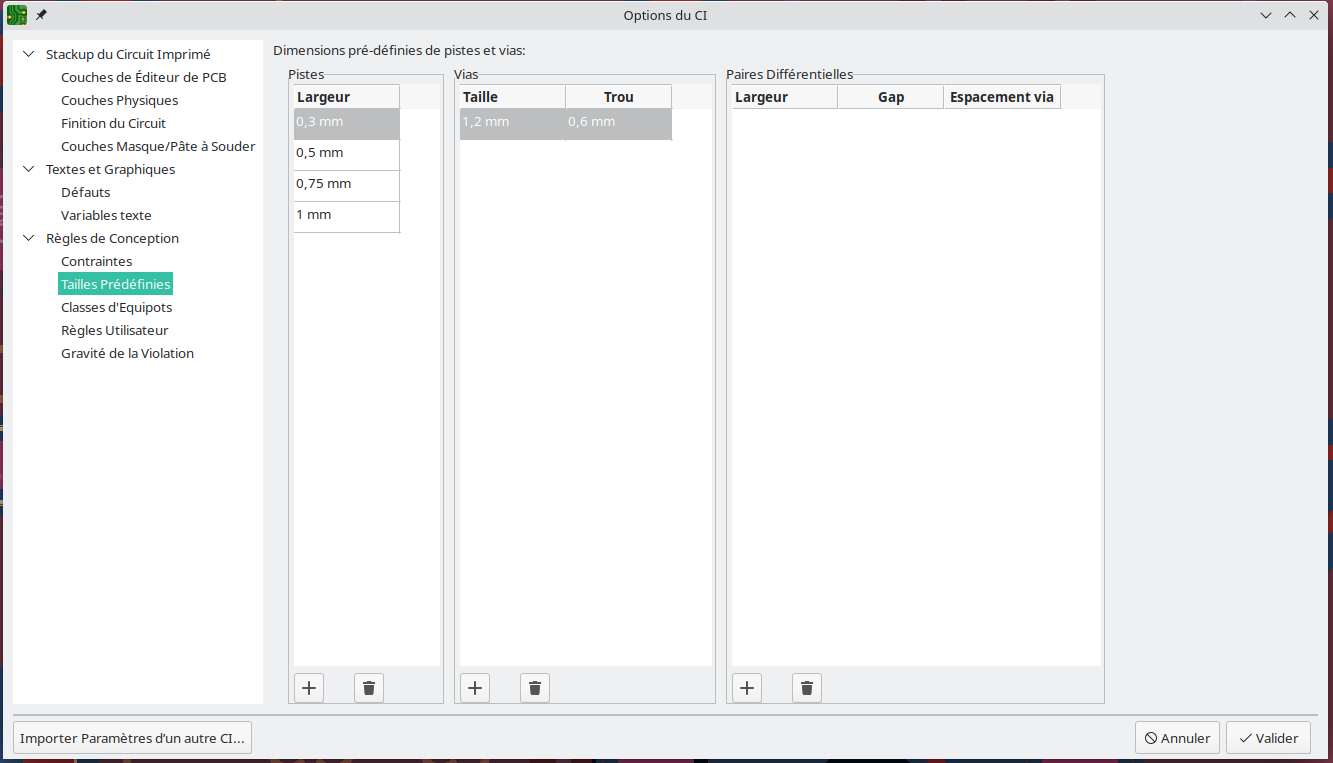
\includegraphics[width=\linewidth]{figures/kicad26.png}
    \end{center}

	\question Dans \emph{Board Stackup > Solder Mask/Paste}, configurez selon la figure suivante:
	\begin{center}
        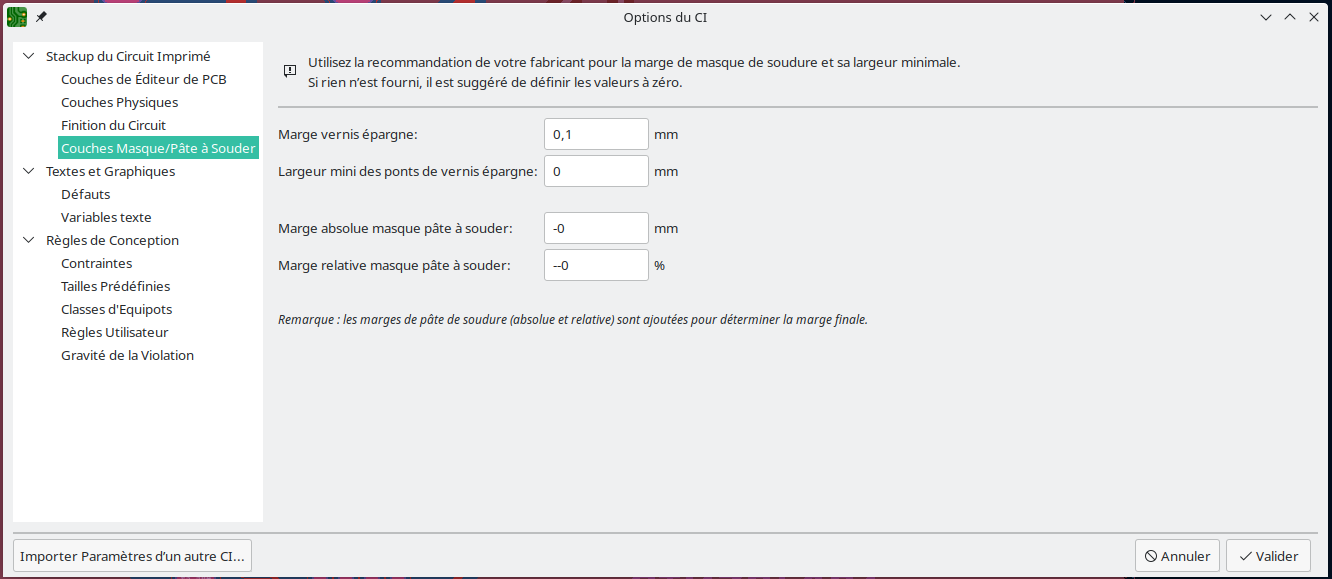
\includegraphics[width=\linewidth]{figures/kicad30.png}
    \end{center}

\newpage

	\question Dans le panneau de droite, cliquez sur F.Cu. 
	Ensuite, cliquez sur \texttt{Place > Add Filled Zone...}.
	Choisissez le signal GND.
	Tracer un rectangle englobant tout le circuit.

	\begin{center}
        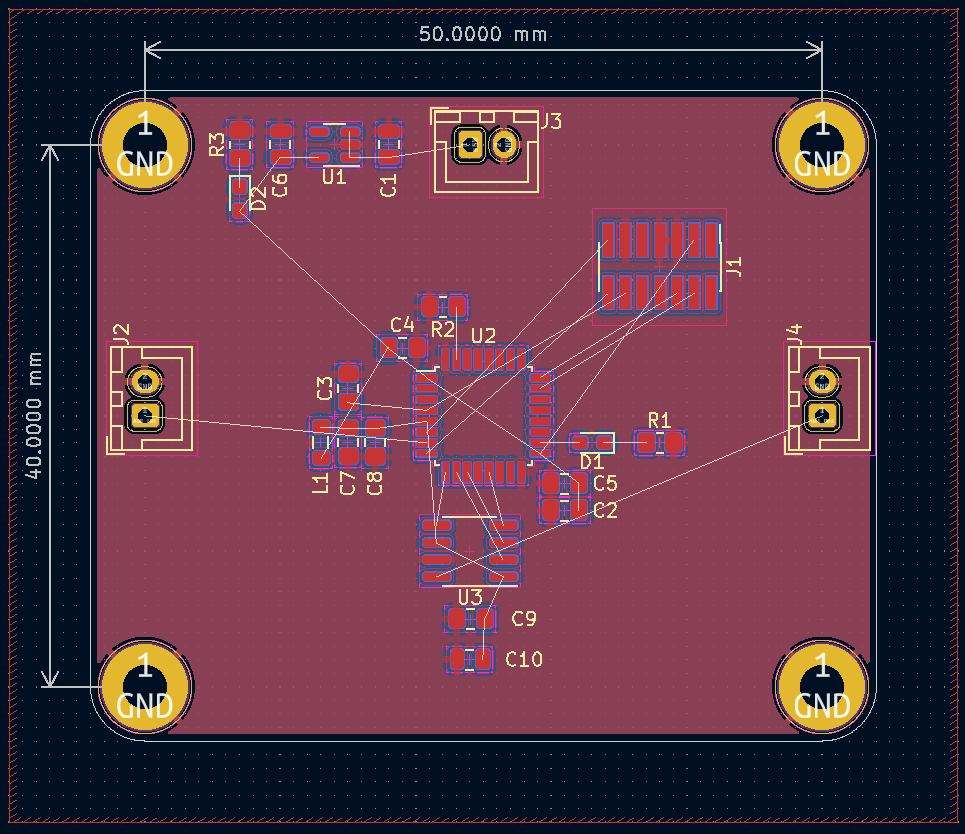
\includegraphics[width=.8\linewidth]{figures/kicad28.png}
    \end{center}

	\question Faites de même avec la couche B.Cu.

	\question Pour pouvoir router, cliquez sur \texttt{View > Drawing Mode > Draw Zone Outlines}. (Aussi présent dans le menu de gauche.)

	\question Routez la carte. Les pistes de 0.3mm sont reservées aux signaux. Les pistes de 0.5mm, 0.75mm et 1mm sont à utiliser pour les alimentations.
	C'est encore une étape assez longue. N'hésitez pas à supprimer des pistes déjà routées pour trouver de meilleures solutions.
	Pensez également à replacer certains composants pour faciliter le routage.
\end{questions}

	\vspace{2em}
	Félicitations vous avez routé la carte! Faites valider le routage par l'enseignant.

	\newpage
\subsection{Génération des fichiers de fabrication}
\begin{questions}
	\question Cliquez sur \emph{File > Fabrication Outputs > Gerbers (.gbr)}.
	\question Configurer selon la figure suivante:
	\begin{center}
        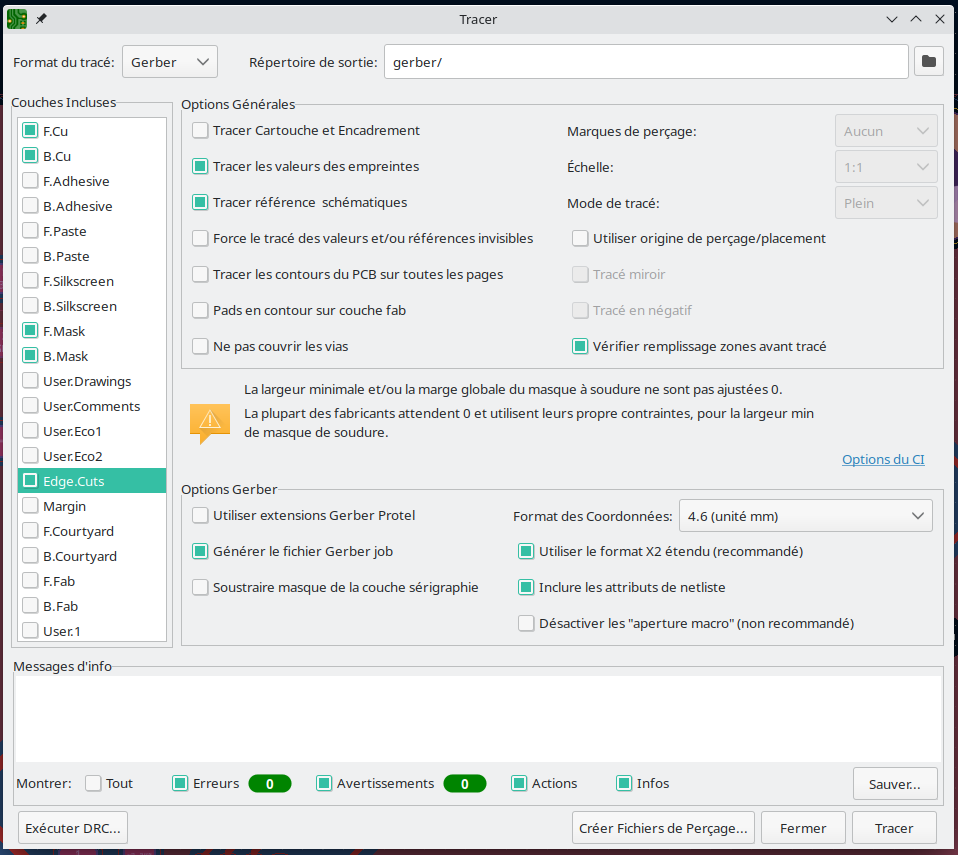
\includegraphics[scale=.6]{figures/kicad31.png}
    \end{center}
	\question Cliquez sur \emph{Créer Fichiers de Perçage...}
	\newpage
	\question Configurer selon la figure suivante:
	\begin{center}
        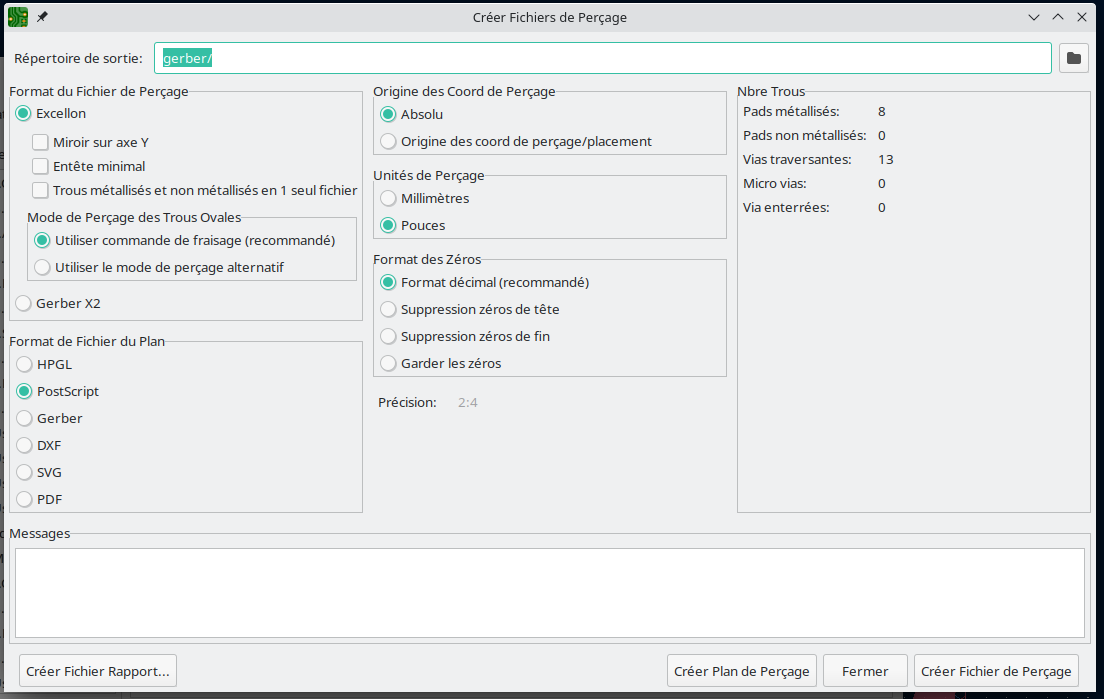
\includegraphics[scale=.6]{figures/kicad32.png}
    \end{center}
	\question Cliquez sur \emph{Créer fichier de perçage}
	\question Cliquez sur \emph{Tracer}
	\question Faites valider. N'oubliez pas de commiter et de pousser sur github.
\end{questions}

\newpage

\section{Écriture du firmware}
La section \emph{Écriture du firmware} est présente avant la section \emph{Assemblage} parce que, arrivés à cette partie du projet, vous n'avez probablement pas encore votre carte.
C'est quelque chose d'assez courant dans une phase de développement.

Néanmoins, il est quand même possible d'avancer:
\begin{itemize}
	\item On peut tester que le projet compile sur la cible.
	\item On peut valider l'application sur PC ou sur une autre cible (F746 discovery par exemple).
	\item On peut tester les drivers sur une autre cible (F746 ou Nucleo).\\
\end{itemize}

Vous constaterez rapidement que le STM32L021K4 est assez contraint en mémoire RAM et FLASH. 
Ainsi, vous allez souvent chatouiller les limites du microcontrôleur.

Ce point vous imposera quelques contraintes:
\begin{itemize}
	\item Il est hors de question d'utiliser FreeRTOS.
	\item On ne pourra pas utiliser de nombres flottants.
	\item On ne pourra pas écrire de structure de drivers trop complexe (on essaiera quand même d'écrire du code propre).
	\item On ne pourra pas utiliser les fonctions de haut niveau de la HAL.
		\begin{itemize}
			\item On pourra quand même utiliser les Low Layer (LL) drivers.
		\end{itemize}
	\item On devrait pouvoir utiliser le shell. %TODO git
\end{itemize}

\newpage
\subsection{Activation des LL drivers}
\begin{questions}
	\question Dans le fichier \texttt{.ioc}, dans \emph{Project Manager > Advanced Settings}, choisissez LL pour tous les périphériques.
	\begin{center}
		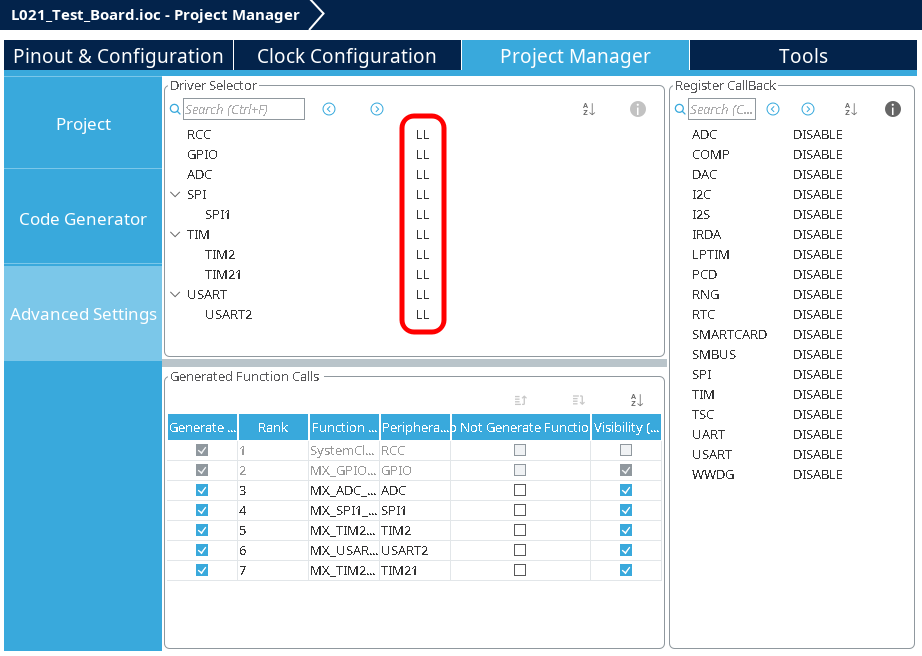
\includegraphics[width=.9\linewidth]{figures/cube02.png} 
	\end{center}
	\question Regardez les fichiers générés. Quelles sont les différences?
	\question Les fonctions de la LL sont des accès directs aux registres. 
	Il faudra chercher de la documentation. Vous aurez besoin du \emph{Reference Manual} du STM32L021K4 et de la documentation de la HAL STM32L0 (ou lire le code à l'aide de la touche F3 sur CubeIDE).
	\question Que signifie \mintinline{C}{__STATIC_INLINE}? 
	\question Et pourquoi y a-t-il du code dans un .h alors que Môssieur Fiack vous a expressément demandé de pas le faire? (Les deux questions sont peut-être liés, va savoir)
\end{questions}

\newpage
\subsection{LED simple}
\begin{questions}
	\question Configurer le timer de la LED pour obtenir une fréquence de découpage d'1kHz et une résolution de 8bits. 
	Ça veut dire que Counter period vaut 255.
	\question Quelle valeur donner au prescaler?
	\question Créez une paire de fichiers \texttt{Led.c} / \texttt{Led.h} dans \texttt{Core/Src} et \texttt{Core/Inc} respectivement
	\question Écrivez les trois fonctions suivantes :
	\begin{minted}{C}
// Démarre le timer
void LedStart(void);
// Configure le rapport cyclique de la PWM entre 0 et 255
void LedSetValue(uint8_t val);
// À chaque appel, cette fonction incrémente la luminosité de la LED
// Arrivé à la valeur maximale, chaque appel décrémente la LED
void LedPulse(void);
	\end{minted}
	\question La fonction LEDPulse demande de conserver la luminosité entre deux appels, ainsi qu'une variable permettant de savoir si on incrémente ou décrémente.
	\question Si vous n'avez pas peur, vous pouvez stocker ses informations, ainsi que celles relative aux timer, dans une structure.
	Si c'est pas clair, n'hésitez pas à demander, votre enseignant est payé pour ça.
	\question Pour un premier test, la fonction LEDPulse pourra être appelée dans une boucle infinie, accompagnée d'un délai.
	Ça pourrait ressembler à ça:
	\begin{minted}{C}
/* USER CODE BEGIN WHILE */
LedStart();
while (1) {
    // Dans cet exemple, LedPulse fait appel à LedSetValue
    LedPulse();
    LL_mDelay(1);
    /* USER CODE END WHILE */
    
    /* USER CODE BEGIN 3 */
}
/* USER CODE END 3 */
	\end{minted}
	\question Vous ne pouvez pas tester le code, n'hésitez pas à le faire valider par votre enseignant.
\end{questions}

\newpage
\subsection{LED avec timer}
\begin{questions}
	\question Activer le timer qui n'est pas utilisé par la PWM de la LED.
	\question Configurez le pour qu'il déclenche une interruption toutes les milli-secondes.
	\question Quelles sont les valeurs de PSC et de ARR?
	\question Créez une paire de fichiers \texttt{TimeBase.c} / \texttt{TimeBase.h}
	\question Écrivez une fonction:
	\begin{minted}{C}
void TimeBaseStartIT(void);
	\end{minted}
	\question Où se situe la routine de service d'interruption?
	\question Que manque-t-il par rapport au code généré par la HAL? 
	\question En quoi est-ce catastrophique? 
	\question Que faire?
	\question Déplacer l'appel à la fonction \mintinline{C}{LedPulse()} dans la routine de service du timer. 
	\question Vous ne pouvez pas tester le code, n'hésitez pas à le faire valider par votre enseignant.
\end{questions}

\subsection{UART, un simple echo}
\begin{questions}
	\question La configuration de l'UART est probablement correcte par défaut. Vérifiez quand même, ça ne coûte pas grand chose.
	\question Créez une paire de fichiers \texttt{Serial.c} / \texttt{Serial.h}
	\question Écrivez les fonctions suivantes:
	\begin{minted}{C}
// Cette fonction pourra être utilisée par le Shell v0.4
uint8_t SerialTransmit(char * pData, uint16_t Size);
// Dans cet exemple, on fait du polling, et c'est pas très grave
char SerialReceiveChar(void);
	\end{minted}
	\question Écrivez un test permettant de réaliser un echo. Ça pourrait ressembler à ça:
	\begin{minted}{C}
/* USER CODE BEGIN WHILE */
while (1) {
    char ch = SerialReceiveChar();
    SerialTransmit(ch, 1);
    /* USER CODE END WHILE */

    /* USER CODE BEGIN 3 */
}
/* USER CODE END 3 */
	\end{minted}
	\question Une erreur s'est glissée dans le code précédent, saurez-vous la retrouver?
	\question Vous ne pouvez pas tester le code, n'hésitez pas à le faire valider par votre enseignant.
\end{questions}

\subsection{UART et Shell}
\begin{questions}
	\question Ajoutez le Shell que vous avez utilisé en TP de FreeRTOS, ou utilisez la toute dernière version disponible à cette adresse : \url{https://github.com/lfiack/mcuLib/tree/main/Middleware/Shell}
	\question Le code pourrait ressembler à quelque chose comme ça:
	\begin{minted}{C}
    [...]
/* USER CODE BEGIN PV */
hShell_t hShell;
/* USER CODE END PV */
    [...]
int main(void) {
        [...]
    /* USER CODE BEGIN 2 */
    ShellInit(&hShell, &SerialTransmit);
    /* USER CODE END 2 */
        [...]
    /* USER CODE BEGIN WHILE */
    while (1) {
        char c = SerialReceiveByte();
        ShellProcess(&hShell, c);
        /* USER CODE END WHILE */

        /* USER CODE BEGIN 3 */
    }
    /* USER CODE END 3 */
}

	\end{minted}
	\question Vous ne pouvez pas tester le code, n'hésitez pas à le faire valider par votre enseignant.
\end{questions}

\subsection{DAC, génération de signaux}
\begin{questions}
	\question Configurer le SPI dans le fichier \texttt{.ioc}
	\question Créez une paire de fichiers \texttt{AnalogOut.c} / \texttt{AnalogOut.h}
	\question Écrivez les fonctions suivantes :
	\begin{minted}{C}
void AnalogOutInit(void);
void AnalogOutConvert(uint16_t value);
void AnalogOutPulse(uint16_t increment);
	\end{minted}
	Comme \mintinline{C}{LedPulse()}, à chaque appel, cette fonction incrémente la valeur à envoyer au DAC jusqu'à une valeur maximale. 
	Arrivé à la valeur maximale, chaque appel décrémente cette valeur.
	Ça devrait générer un signal triangle.
	\question Testez avec le timer \mintinline{C}{TimeBase}. Augmenter la fréquence d'interruption du timer, par exemple à 32kHz.
	\question Vous ne pouvez pas tester le code, n'hésitez pas à le faire valider par votre enseignant.
\end{questions}

\subsection{ADC, un bypass analogique}
\begin{questions}
	\question Vous pouvez garde la configuration par défaut de l'ADC.
	\question Créez une paire de fichiers \texttt{AnalogIn.c} / \texttt{AnalogIn.h}
	\question Écrivez les fonctions suivantes:
	\begin{minted}{C}
void AnalogInInit(void);
void AnalogInStartConversion(void);
// Cette fonction fait du polling, même si c'est pas bien
uint16_t AnalogInGetValue(void);
	\end{minted}
	\question Dans la routine de service d'interruption du timer, lire la valeur analogique, et la renvoyer telle quelle sur le DAC. Ça pourrait ressembler à ça:
	\begin{minted}{C}
void TIM21_IRQHandler(void) {
    [...]

    AnalogInStartConversion();
    uint16_t ADCValue = AnalogInGetValue();
    uint16_t DACValue = ADCValue;
    AnalogOutConvert(DACValue);
}
	\end{minted}
	\question Vous ne pouvez pas tester le code, n'hésitez pas à le faire valider par votre enseignant.

\end{questions}

\newpage
\subsection{Filtre RC}
\begin{questions}
	\question Quelle est la fréquence d'échantillonnage maximale atteignable par l'ADC? Par le DAC?\\
	\begin{minipage}[c]{.26\linewidth}
        \center
		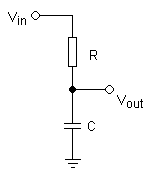
\includegraphics[width=\linewidth]{figures/rc.png}
    \end{minipage}
    \hfill
    \begin{minipage}[c]{.66\linewidth}
		\vspace{1em}
		\question Écrivez l'équation différentielle régissant le filtre RC ci-contre.
		Mettre l'équation sous la forme suivante:
		$$V_{in} = X \cdot \frac{dV_{out}(t)}{dt} + Y \cdot V_{out}$$
		\question Écrivez l'équation de récurrence correspondante. On peut remplacer $\frac{dV(t)}{dt}$ par $\frac{V[n] - V[n-1]}{T}$.
		Pour faciliter le codage, on utilisera plutôt l'expression suivante:
		$$f_s \cdot \left(V[n] - V[n-1]\right)$$
		Avec $f_s$ la fréquence d'échantillonnage.
		\vspace{1em}
    \end{minipage}
	Mettre sous la forme suivante:
	$$V_{out}[n] = \frac{A \cdot V_{in}[n] + B \cdot V_{out}[n-1]}{D}$$
	\question Donnez les expressions de $A$, $B$ et $D$.
		Remplacez $RC$ par $\frac{1}{2 \cdot \pi \cdot f_c}$.
	\question On travaillera avec une fréquence d'échantillonnage de 32kHz. Combien de cycles processeurs disposons-nous pour traiter chaque échantillon?
	\question Créez une paire de fichiers \texttt{RCFilter.c} / \texttt{RCFilter.h}
	\question Créez la structure suivante dans \texttt{RCFilter.h}:
	\begin{minted}{C}
typedef struct {
    uint32_t coeffA;
    uint32_t coeffB;
    uint32_t coeffD;
    uint16_t out_prev;
} hRCFilter_t;
	\end{minted}
    \question Écrivez les fonctions suivantes:
    \begin{minted}{C} 
// Calcule les coefficients A, B et D
// Et les stocke dans la structure
void RCFilterInit(hRCFilter_t * hRCFilter, 
        uint16_t cutoffFrequency, uint16_t samplingFrequency);
// Implémente l'équation de récurrence
// Faites attention au type des différentes variables
uint16_t RCFilterUpdate(hRCFilter_t * hRCFilter, uint16_t input);
    \end{minted}
	\question Ajoutez une fonction au Shell pour modifier la fréquence de coupure.

	\question Vous ne pouvez pas tester le code, n'hésitez pas à le faire valider par votre enseignant.
\end{questions}


\newpage

\section{Assemblage}
\begin{questions}
	\question Avant de souder, faites un test de continuité. Vérifiez également qu'il n'y ait pas de courts circuits.
	\question Soudez les composants:
	\begin{itemize}
		\item Commencez par les circuits intégrés (STM32, DAC, LDO)
		\item Continuez avec les petits composants (Condensateurs, résistances, LED)
		\item Soudez ensuite le connecteur SWD
		\item Finissez avec le connecteur 4 pin au bottom de la carte.
	\end{itemize}
	\question Alimentez la carte. Régler une limitation de courant de 100mA au niveau de l'alimentation.
	\question Mesurer les différentes tensions d'alimentation (VDD et VDDA).
	\question Branchez la STLINKV3-Mini et testez la communication, d'abord avec l'outil \emph{stlink-gui} puis en programmant un firmware simple.
	\question Testez ensuite les différents firmwares:
	\begin{parts}
		\part LED simple
		\part LED + timer
		\part UART
		\part UART + Shell
		\part DAC avec timer
		\part Bypass ADC -> DAC.
		\textbf{Attention niveaux de tension!} Ne pas descendre en dessous de 0V, ne pas monter au dessus de 3,3V. Vérifier à l'oscilloscope avant d'appliquer le signal.
		\part Filtre RC
	\end{parts}
\end{questions}
\end{document} 
